% main.tex
% Fichero principal de transparencias (incluye a todos los demás).

% Compilar a .pdf con LaTeX (pdflatex)
% Es necesario instalar Beamer (paquete latex-beamer en Debian)
%

% Gráficos:
% Los gráficos pueden suministrarse en PNG, JPG, TIF, PDF, MPS
% Los EPS deben convertirse a PDF (usar epstopdf)
%
%\documentclass[17pt,aspectratio=169,hyperref={pdfusetitle,colorlinks,citecolor=blue,linkcolor=blue,urlcolor=blue}]{beamer}
\documentclass[17pt,aspectratio=169,hyperref={pdfusetitle,colorlinks,allcolors=olive}]{beamer}
\usetheme[orchid]{Hannover}
\beamertemplatenavigationsymbolsempty
\setbeamertemplate{headline}{}
\useoutertheme{infolines}

\usepackage{lmodern}
\usepackage[spanish]{babel}
\usepackage[utf8]{inputenc}
\usepackage{graphics}
\usepackage{multicol}
%\usepackage{amssymb} % Simbolos matematicos
%\usepackage[pdfusetitle]{hyperref}

%\usepackage{chronosys}

%% two slides per page
%\usepackage{pgfpages}
%\pgfpagesuselayout{2 on 1}[a4paper,border shrink=5mm]
%\usepackage{tikz}

\newcommand\YUGE{\fontsize{48}{60}\selectfont}

\newcommand{\secimage}{figs/bookpages}
\AtBeginSection[]
{
  {
    \usebackgroundtemplate{\includegraphics[width=\paperwidth,height=\paperheight]{\secimage}}
    \begin{frame}<beamer>

      \begin{center}
        {\YUGE\bf\insertsection}
      \end{center}
    \end{frame}
  }
  \renewcommand{\secimage}{figs/bookpages}
}

\newcommand{\F}{\mathcal F}
\newcommand{\Co}{\mathcal C}
\newcommand{\lag}{\mathcal L}
\newcommand{\fideal}{\func{ideal}}
\newcommand{\fdelta}{\func{delta}}
\newcommand{\fagg}{\func{agg}}
\newcommand{\tuple}[1]{{\left( #1 \right)}}
\newcommand{\func}[1]{\mathbf{#1}}
\newcommand{\powerset}[1]{\mathbb P({#1})}
\newcommand{\outdateness}{\func{outdateness}}
\newcommand{\techlag}{\func{techlag}}
\newcommand{\components}{\func{components}}

\title[Technical Lag Outdateness]{Characterizing outdateness with technical lag}
%\subtitle{}
\author[Jesus M. Gonzalez-Barahona]{Jesus M. Gonzalez-Barahona}
\institute[URJC]{Universidad Rey Juan Carlos \\
  @jgbarah ~~~~~ \url{https://jgbarah.github.io/presentations}}

\date{3rd Intl. Workshop on Software Health \\
(SoHeal 2020) July 3rd 2020}

\begin{document}

%\begin{frame}[label=firstframe]
\begin{frame}
  \maketitle
\end{frame}



%%-----------------------------------------
\begin{frame}
  \frametitle{The plan}

  \tableofcontents

\end{frame}

%%-----------------------------------------
%%-----------------------------------------
\section{Context}

%%-----------------------------------------
\begin{frame}[fragile]
  \frametitle{Context}

  Applications are composed of tens, \\
  maybe hundreds of components \\

  \vspace{1cm}

  Each component is normally used as a package \\
  ...and that package has a story \\
\end{frame}

%%-----------------------------------------
\begin{frame}[fragile]
  
  \begin{center}
  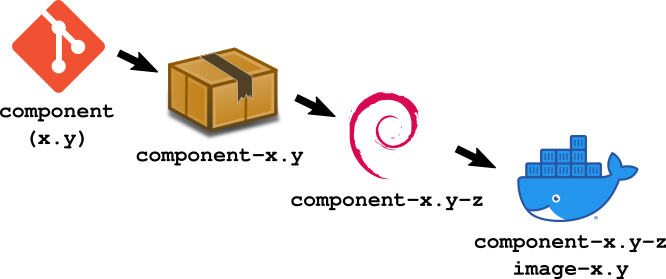
\includegraphics[width=11cm]{figs/component-pkgs}
  \end{center}
    
\end{frame}

%%-----------------------------------------
\begin{frame}[fragile]
  
  \begin{center}
    {\Huge Main goal:} \\
    \vspace{1cm}
    \large How can we compute outdateness \\
    for an application \\
    considering all its components? \\
  \end{center}
    
\end{frame}

%%-----------------------------------------
\begin{frame}[fragile]
  
  \begin{center}
    {\Large Secondary goals:}
    \vspace{.5cm}
    \begin{itemize}
    \item Metrics useful for several situations
    \item Factors imposing a lower bound on outdateness
    \item Metrics for characterizing an ecosystem
    \end{itemize}

    \vspace{1cm}

    {\Large How:}\\
    \vspace{.5cm}
    Technical lag framework \\
   
  \end{center}
    
\end{frame}

%%-----------------------------------------
%%-----------------------------------------
\section{Outdateness}

%%-----------------------------------------
\begin{frame}[fragile]
  \frametitle{Outdateness of an application}

  How outdated it is, \\ due to its components being outdated? \\

  \begin{center}
    {\Large $\Downarrow$}
  \end{center}

  How old are its components \\
  with respect to the latest version \\
  available from upstream? \\
  
\end{frame}


%%-----------------------------------------
\begin{frame}[fragile]
  \frametitle{Idea}

  {\Large Most up to date:} \\
    current master in upstream git repo \\

    \vspace{1cm}
    
    Map all packages to git commits \\
    
\end{frame}

%%-----------------------------------------
\begin{frame}[fragile]
  
y  \begin{center}
  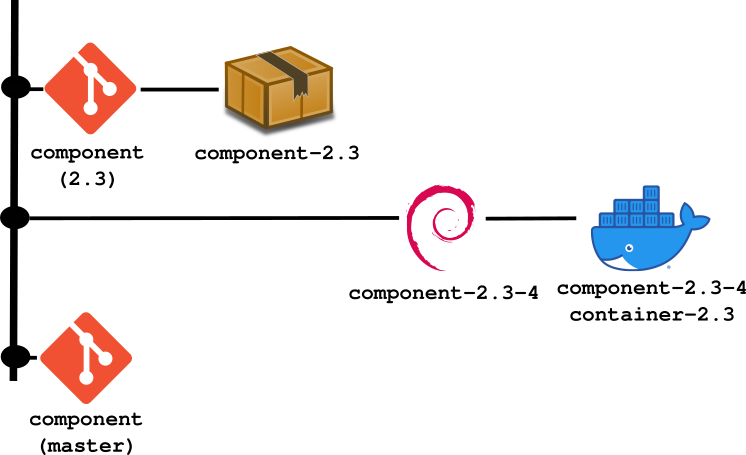
\includegraphics[width=11cm]{figs/component-pkgs-diff}
  \end{center}
    
\end{frame}

%%-----------------------------------------
\begin{frame}[fragile]
  
  \begin{center}
  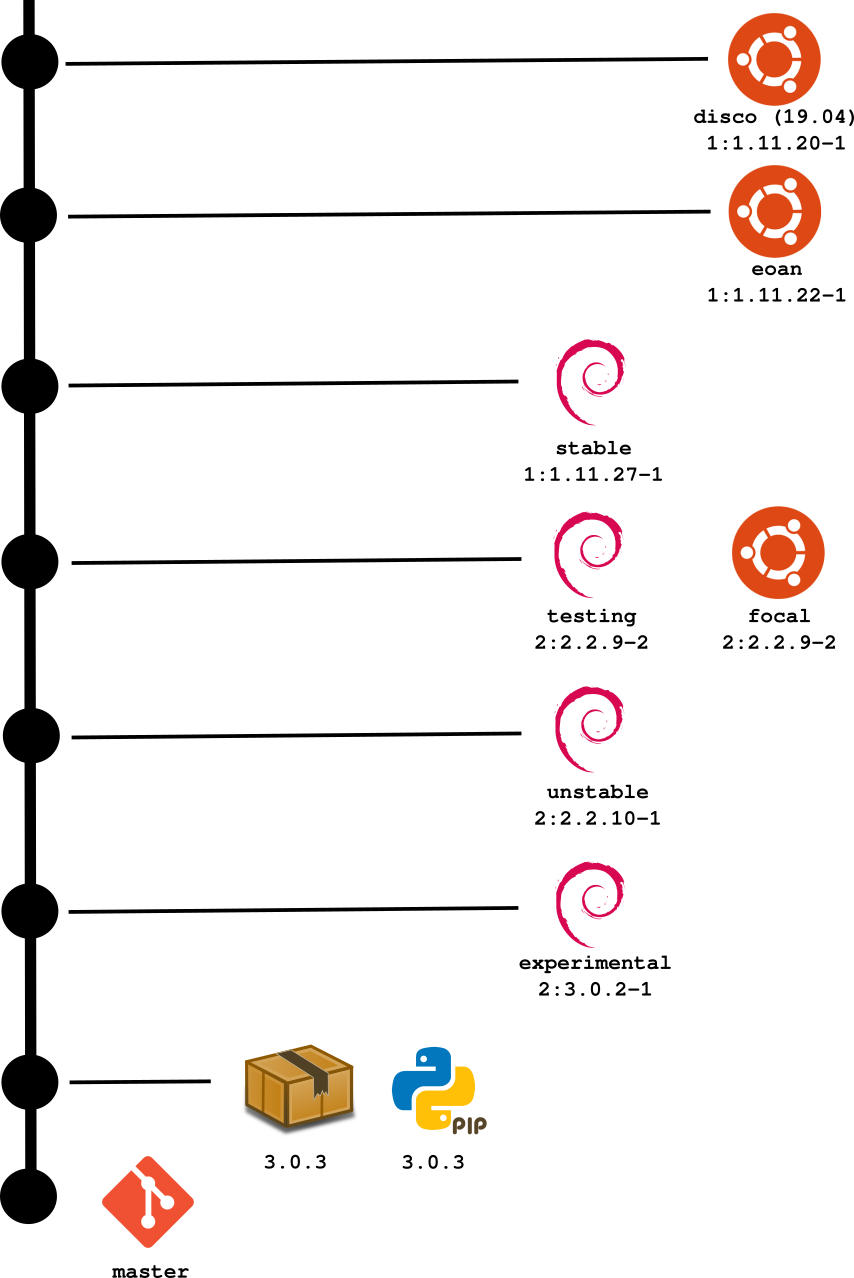
\includegraphics[height=7.5cm]{figs/django-versions}
  \end{center}
    
\end{frame}

%%-----------------------------------------
%%-----------------------------------------
\section{Outdateness as technical lag}


%%-----------------------------------------
\begin{frame}[fragile]
  \frametitle{Technical lag}
  
{\small
$\F = \tuple{\Co, \lag, \fideal, \fdelta, \fagg}$

  \begin{itemize}
\item $\Co$ set of component releases
\item $\lag$ set of possible lag values
\item $\fideal: \Co \rightarrow \Co$ function returning the ``most preferred'' component release
\item $\fdelta: \Co \times \Co \rightarrow \lag$ function computing the difference between two component releases
\item $\fagg: \powerset\lag \rightarrow \lag$ function aggregating lag values for a set of components.
\end{itemize}
}
    
\end{frame}


%%-----------------------------------------
\begin{frame}[fragile]
  \frametitle{Computing difference}

  {\large
  Difference between two components \\
  is the difference \\
  between their two most likely commits \\
  in the upstream repo \\
  }
\end{frame}


%%-----------------------------------------
\begin{frame}[fragile]
  \frametitle{Outdateness}

  {\large
    Technical lag \\
    (with previous definition for difference) \\
    between a component \\
    and current upstream master \\
  }
\end{frame}


%%-----------------------------------------
\begin{frame}[fragile]

  Component:
  \begin{center}
  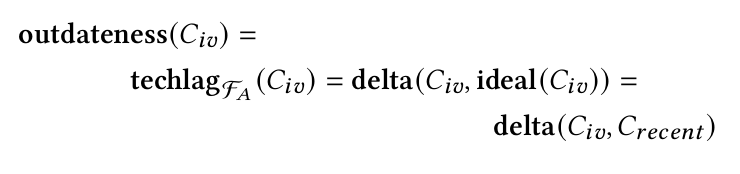
\includegraphics[width=12cm]{figs/outdateness-techlag}
  \end{center}

  Aggregation:
  \begin{center}
  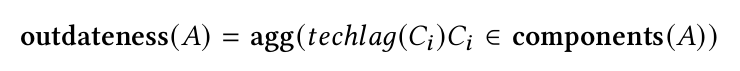
\includegraphics[width=12cm]{figs/outdateness-aggregation}
  \end{center}

  
\end{frame}


%%-----------------------------------------
%%-----------------------------------------
\section{Applications of the model}

%%-----------------------------------------
\begin{frame}[fragile]
  \frametitle{Minimum outdateness}
  
\begin{itemize}
\item Minimum outdateness possible is outdateness of latest package by upstream
\item Influenced by publication practices
\item Different collections, different minimum outdateness for same component
\item Example: Django
\end{itemize}

{\small $Pypi < Debian_{testing} < Ubuntu_{focal} < Debian_{stable}$}

\end{frame}


%%-----------------------------------------
\begin{frame}[fragile]
  \frametitle{Collections}

  \begin{itemize}
  \item Characterizable by mean / median outdateness
  \item Example: LTS, testing, experimental releases
  \item Example: components from Pypi or from Debian
  \item Example: effect of pinning dependencies
  \end{itemize}
\end{frame}


%%-----------------------------------------
\begin{frame}[fragile]
  \frametitle{Applications}

  \begin{itemize}
  \item For an application, mean / median \\
    outdateness can be computed \\
    per collection \\
    (constrained by dependencies) \\
  \item Decisions on dependencies for a certain collection
  \end{itemize}
\end{frame}


%%-----------------------------------------
\begin{frame}[fragile]
  \frametitle{Comparing collections}

  \begin{itemize}
  \item Absolute outdateness
  \item Dependency outdateness
  \end{itemize}
\end{frame}


\section{Final notes}

%%-----------------------------------------
\begin{frame}[fragile]
  \frametitle{Conclusions}

  Technical lag can be used to precisely define outdateness

  Outdateness can be used to:
  
  \begin{itemize}
  \item compute impact of release policies
  \item compare collections
  \item compute the effect of constraints on dependencies
  \item make decisions on dependencies, collections to use
  \end{itemize}
\end{frame}



%%-----------------------------------------
\begin{frame}[fragile]
  \frametitle{Credits}

  
\includegraphics[width=1.5cm]{figs/bookpages}
  {\small \href{https://pixabay.com/en/book-reading-library-literature-1261800/}{Book}, by NikolayFrolochkin, Pixabay. \\ License: Creative Commons CC0 \\}


\end{frame}



\frame{
~
\vspace{1cm}

\begin{flushright}


\includegraphics[width=2.2cm]{figs/by-sa}
 \\

\begin{footnotesize}
\copyright 2020 Jesus M. Gonzalez-Barahona. \\

\vspace{.4cm}

Some rights reserved. This document is distributed under the terms of the Creative Commons License ``Attribution-ShareAlike 4.0'',
available in \\
{\scriptsize \url{http://creativecommons.org/licenses/by-sa/4.0/}} \\

\vspace{.4cm}

This document (including source) is available from
\url{https://jgbarah.github.io/presentations}

\end{footnotesize}
\end{flushright}

}
%%

%\againframe{firstframe}

\end{document}
